\documentclass[a4paper,twoside]{article}
\usepackage{blindtext}  
\usepackage{geometry}

% Chinese support
\usepackage[UTF8, scheme = plain]{ctex}

% Page margin layout
\geometry{left=2.3cm,right=2cm,top=2.5cm,bottom=2.0cm}


\usepackage{listings}
\usepackage{xcolor}
\usepackage{geometry}
\usepackage{amsmath}
\usepackage{float}
\usepackage{hyperref}

\usepackage{graphics}
\usepackage{graphicx}
\usepackage{epsfig}
\usepackage{float}
\usepackage{caption}
\usepackage{subcaption}

\usepackage{algorithm}
\usepackage[noend]{algpseudocode}

\usepackage{booktabs}
\usepackage{threeparttable}
\usepackage{longtable}
\usepackage{tikz}
\usepackage{multicol}

% cite package, to clean up citations in the main text. Do not remove.
\usepackage{cite}

\usepackage{color,xcolor}

%% The amssymb package provides various useful mathematical symbols
\usepackage{amssymb}
%% The amsthm package provides extended theorem environments
\usepackage{amsthm}
\usepackage{amsfonts}
\usepackage{enumerate}
\usepackage{enumitem}
\usepackage{listings}
\usepackage{minted}


\usepackage{indentfirst}
\setlength{\parindent}{2em} % Make two letter space in the first paragraph
\usepackage{setspace}
\linespread{1.5} % Line spacing setting
\usepackage{siunitx}
\setlength{\parskip}{0.5em} % Paragraph spacing setting

% \usepackage[contents =22920202204622, scale = 10, color = black, angle = 50, opacity = .10]{background}

\renewcommand{\figurename}{图}
\renewcommand{\listingscaption}{代码}
\renewcommand{\tablename}{表格}
\renewcommand{\contentsname}{目录}
\floatname{algorithm}{算法}

\graphicspath{ {images/} }

%%%%%%%%%%%%%
\newcommand{\StudentNumber}{22920202204622}  % Fill your student number here
\newcommand{\StudentName}{熊恪峥}  % Replace your name here
\newcommand{\PaperTitle}{实验(三)指令调度和分支延迟}  % Change your paper title here
\newcommand{\PaperType}{计算机系统结构实验} % Replace the type of your report here
\newcommand{\Date}{2023年4月19日}
\newcommand{\College}{信息学院}
\newcommand{\CourseName}{计算机系统结构}
%%%%%%%%%%%%%

%% Page header and footer setting
\usepackage{fancyhdr}
\usepackage{lastpage}
\pagestyle{fancy}
\fancyhf{}
% This requires the document to be twoside
\fancyhead[LO]{\texttt{\StudentName }}
\fancyhead[LE]{\texttt{\StudentNumber}}
\fancyhead[C]{\texttt{\PaperTitle }}
\fancyhead[R]{\texttt{第{\thepage}页,共\pageref*{LastPage}页}}


\title{\PaperTitle}
\author{\StudentName}
\date{\Date}

\algnewcommand\algorithmicinput{\textbf{Input:}}
\algnewcommand\algorithmicoutput{\textbf{Output:}}
\algnewcommand\Input{\item[\algorithmicinput]}%
\algnewcommand\Output{\item[\algorithmicoutput]}%

\usetikzlibrary{positioning, shapes.geometric}

\begin{document}
	
%%%%%%%%%%%%%%%%%%%%%%%%%%%%%%%%%%%%%%%%%%%%
\makeatletter % change default title style
\renewcommand*\maketitle{%
	\begin{center} 
		\bfseries  % title 
		{\LARGE \@title \par}  % LARGE typesetting
		\vskip 1em  %  margin 1em
		{\global\let\author\@empty}  % no author information
		{\global\let\date\@empty}  % no date
		\thispagestyle{empty}   %  empty page style
	\end{center}%
	\setcounter{footnote}{0}%
}
\makeatother
%%%%%%%%%%%%%%%%%%%%%%%%%%%%%%%%%%%%%%%%%%%%
	
	
\thispagestyle{empty}

\vspace*{1cm}

\begin{figure}[htb]
	\centering
	
\includegraphics[width=4.0cm]{logo.png}
\end{figure}

\vspace*{1cm}

\begin{center}
	\Huge{\textbf{\PaperType}}
	
	\Large{\PaperTitle}
\end{center}

\vspace*{1cm}

\begin{table}[H]
	\centering	
	\begin{Large}
		\renewcommand{\arraystretch}{1.5}
		\begin{tabular}{p{3cm} p{5cm}<{\centering}}
			姓\qquad 名 & \StudentName  \\
			\hline
			学\qquad号 & \StudentNumber \\
			\hline
			日\qquad期 & \Date  \\
			\hline
			学\qquad院 & \College  \\
			\hline
			课程名称 & \CourseName  \\
			\hline
		\end{tabular}
	\end{Large}
\end{table}

\newpage

\title{
	\Large{\textcolor{black}{\PaperTitle}}
}
	
	
\maketitle
	
\tableofcontents
 
\newpage
\setcounter{page}{1}

\begin{spacing}{1.2}

\section{实验目的}

\begin{enumerate}
	\item 加深对循环级并行性、指令调度技术、循环展开技术以及寄存器换名技术的理解;
	\item 熟悉用指令调度技术来解决流水线中的数据相关的方法;
	\item 了解指令调度、循环展开等技术对CPU性能的改进。
\end{enumerate}

\section{实验内容}

\subsection{用指令调度技术解决流水线中的结构冲突与数据冲突}

调度前,关闭定向功能,执行结果如图~\ref{fig:beforesched}。
总周期33,RAW6次,WAW2次。

\begin{figure}[htb]
	\centering
	\begin{subfigure}[b]{0.4\textwidth}
		\centering
		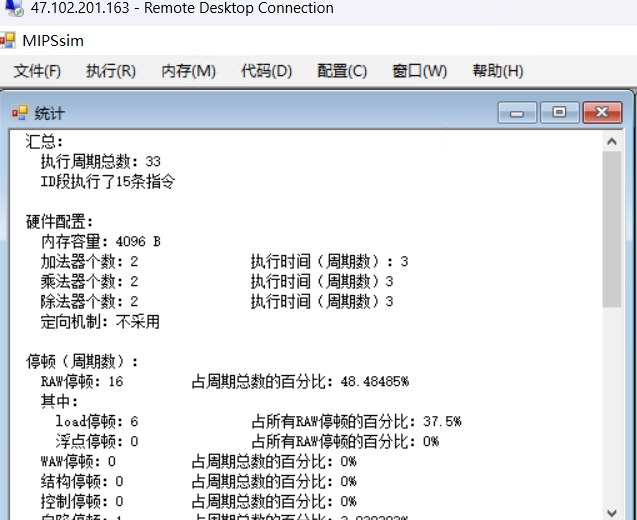
\includegraphics[width=0.9\textwidth]{images/scheafter.png}
		\caption{调度前}
		\label{fig:beforesched}
	\end{subfigure}
	\begin{subfigure}[b]{0.4\textwidth}
		\centering
		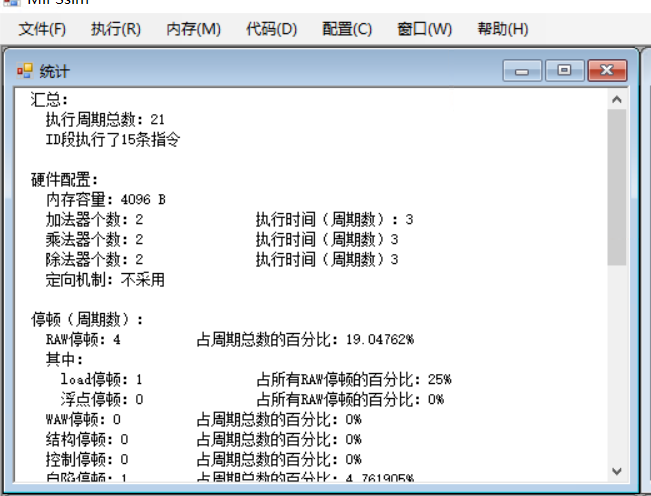
\includegraphics[width=0.9\textwidth]{images/schebefore.png}
		\caption{调度后}
		\label{fig:aftersched}
	\end{subfigure}
\end{figure}

可以发现代码中1、11、12;1、2、3;1,4;1,5,6;1,7;等行需要进行调度以消除冲突,为此,可以把有冲突的
指令放置在较远的位置,这样就可以减少冲突的发生。
进行调度之后代码如代码~\ref{code:aftersched}所示,总周期减少到了21,RAW减少到了4次,WAW减少到了0次。

\begin{listing}[htb]
	\caption{修改后}
	\label{code:aftersched}
	\inputminted{nasm}{../code/after_schedule.s}
\end{listing}

因此,加速比如\eqref{eq:ssched}。
\begin{equation}
	\label{eq:ssched}
	S=\frac{33}{21} = 1.571
\end{equation}

\clearpage

\subsection{用延迟分支减少分支指令对性能的影响}

通过菜单中“配置”、“延迟槽”选项关闭分支延迟,执行结果如图~\ref{fig:nodelay},
时钟周期如图~\ref{fig:nodelayinst}。可以发现在分支指令中进行了较多的停顿。
总共执行了38个周期。

\begin{figure}[htb]
	\centering
	\begin{subfigure}[b]{0.4\textwidth}
		\centering
		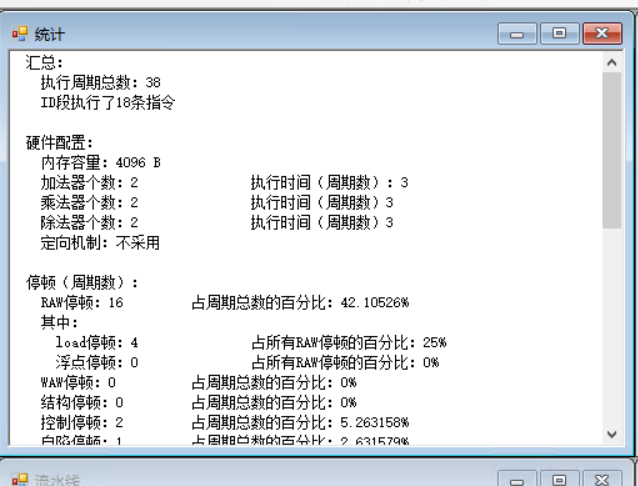
\includegraphics[width=0.9\textwidth]{images/delaybefore.png}
		\caption{不使用延迟}
		\label{fig:nodelay}
	\end{subfigure}
	\begin{subfigure}[b]{0.4\textwidth}
		\centering
		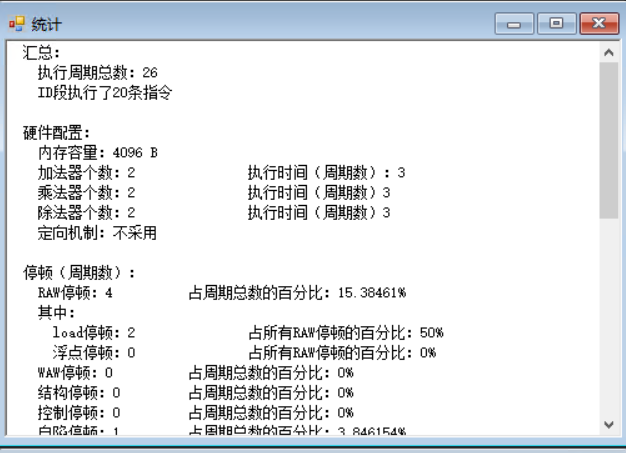
\includegraphics[width=0.9\textwidth]{images/delayafter.png}
		\caption{使用延迟}
		\label{fig:delay}
	\end{subfigure}
	\begin{subfigure}[b]{0.4\textwidth}
		\centering
		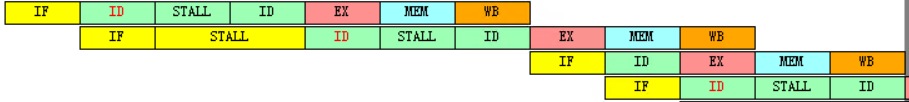
\includegraphics[width=0.9\textwidth]{images/tdelaybefore.png}
		\caption{不使用延迟的时钟周期}
		\label{fig:nodelayinst}
	\end{subfigure}
	\begin{subfigure}[b]{0.4\textwidth}
		\centering
		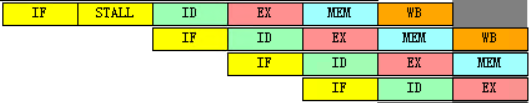
\includegraphics[width=0.9\textwidth]{images/tdelayafter.png}
		\caption{使用延迟的时钟周期}
		\label{fig:delayinst}
	\end{subfigure}
\end{figure}

假设延迟槽有一个,将指令\texttt{LW}放入延迟槽中,并通过上述菜单选项打开延迟槽功能,
执行结果如图~\ref{fig:delay},时钟周期如图~\ref{fig:delayinst}。周期总数
降至25,并且从时钟周期看出分支指令的停顿减少了。

\begin{listing}[htb]
	\caption{修改后}
	\label{code:delayedbranch}
	\inputminted{nasm}{../code/delayed_branch.s}
\end{listing}

\clearpage

\subsection{补充实验}

\subsubsection{解决不能使用L.D和S.D的问题}

补充实验中需要用到浮点数加载和写回的指令\texttt{L.D}和\texttt{S.D},然而由于MIPSSim固有的问题,这些指令
直接使用时汇报如图~\ref{fig:ts1}的错误。为了解决这个错误,需要如图~\ref{fig:ts2}启用延时槽,这样这些指令的运行就能正常。
\begin{figure}[htb]
	\centering
	\begin{subfigure}[b]{0.4\textwidth}
		\centering
		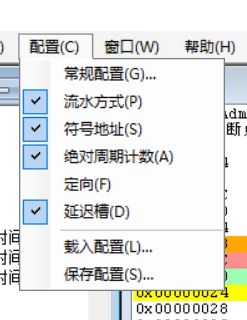
\includegraphics[width=0.4\textwidth]{images/ts1.png}
		\caption{启动延迟槽}
		\label{fig:ts1}
	\end{subfigure}
	\begin{subfigure}[b]{0.4\textwidth}
		\centering
		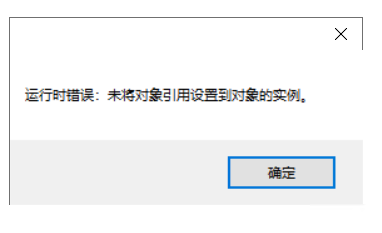
\includegraphics[width=0.9\textwidth]{images/ts2.png}
		\caption{L.D报错信息}
		\label{fig:ts2}
	\end{subfigure}
\end{figure}

\subsubsection{实现}

在补充实验中,我实现了算法~\ref{algo:loop}中的循环,并且为了演示控制冲突,在分支指令后
增加了一个运算操作。代码如代码~\ref{code:first}所示。

\begin{algorithm}
	\caption{实现的循环运算}
	\label{algo:loop}
	\begin{algorithmic}[1]
		\For{$i \in \{ 1,\ldots,16 \}$}
			\State $x[i] \gets x[i] + x[i]$
		\EndFor
	\end{algorithmic}
\end{algorithm}	

\begin{listing}[H]
	\caption{展开前}
	\label{code:first}
	\inputminted{nasm}{../code/before.s}
\end{listing}

执行展开前的代码,结果如图~\ref{fig:beforeunroll}所示,总周期为216,RAW97次,WAW0次。
进行循环展开、并根据指令的换名和调度,然后将指令调度到延迟槽中,得到代码~\ref{code:second}。
结果如图~\ref{fig:afterunroll}所示,

\begin{listing}[H]
	\caption{展开后}
	\label{code:second}
	\inputminted{nasm}{../code/after.s}
\end{listing}


\begin{figure}[htb]
	\centering
	\begin{subfigure}[b]{0.4\textwidth}
		\centering
		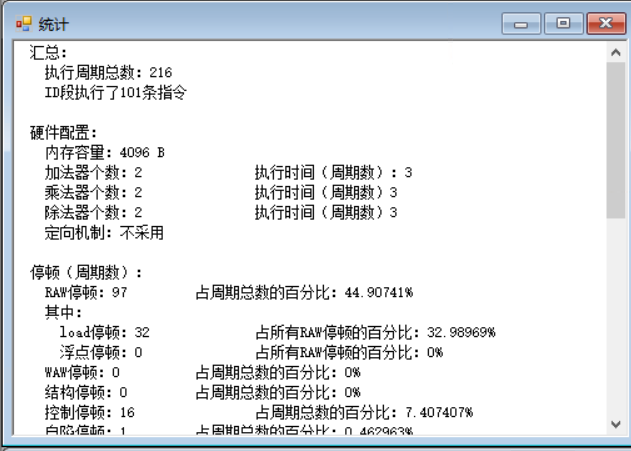
\includegraphics[width=0.9\textwidth]{images/unrollbefore.png}
		\caption{调度前}
		\label{fig:beforeunroll}
	\end{subfigure}
	\begin{subfigure}[b]{0.4\textwidth}
		\centering
		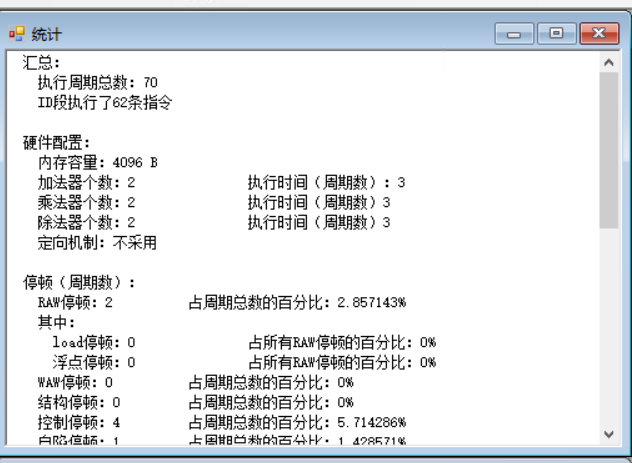
\includegraphics[width=0.9\textwidth]{images/unrollafter.png}
		\caption{调度后}
		\label{fig:afterunroll}
	\end{subfigure}
\end{figure}

思考题:
\begin{enumerate}
	\item \textbf{当定向技术打开和关闭时结果是否有差异?}有,图~\ref{fig:afterunroll}中展示的是
	使用延迟槽的结果。在未使用延迟槽时,时钟周期数稍多。需要注意的是,由于上节提到的问题,
	\emph{在实验时使用了删除了\texttt{L.D}和\texttt{S.D}的程序比较性能}。
	\item \textbf{Stall是否越少越好?}是的,通过减少Stall,可以使程序执行加快提高CPU的性能。当然,
	这可能降低程序的可读性,但是由编译器来完成这项工作时就不会有可读性的问题产生。
\end{enumerate}


\clearpage

\section{实验总结}

在此次实验中,我加深了对循环级并行性、指令调度技术、循环展开技术以及寄存器换名技术的理,
熟悉了用指令调度技术来解决流水线中的数据相关的方法,了解了指令调度、循环展开等技术对CPU性能的改进。
并且通过实际编写代码的方式体验了循环展开减少停顿的方法。

\end{spacing}

\end{document}